\documentclass[journal]{IEEEtran}
\usepackage[a5paper, margin=10mm, onecolumn]{geometry}
\usepackage[cmex10]{amsmath}
\usepackage{amssymb,amsfonts,amsthm}
\usepackage{gvv-book}
\usepackage{gvv}
\usepackage{hyperref}


\begin{document}
\title{10.4.1}
\author{EE25BTECH11025 - Ganachari Vishwambhar}
\maketitle

\textbf{Question}:\\
Find the equations of the tangent and the normal, to the curve $16x^2+9y^2=145$ at the point $\brak{x_1,y_1}$, where $x_1=2$ and $y_1>0$.\\
\textbf{Solution: }\\
Let the point of contact of tangent and conic be $\vec{q}$ and also point of intersection of normal and conic be $\vec{q}$.\\
Given
\begin{align}
    \vec{q}=\myvec{2\\k};k>0
\end{align}

Let the equation of given ellipse in quadratic form be:
\begin{align}
    \vec{x}^\top V\vec{x}+2\vec{u}^\top\vec{x}+f=0\\
\end{align}
where,
\begin{align}
    V=\myvec{\frac{16}{145}&0\\0&\frac{9}{145}}\\
    \vec{u} = \myvec{0\\0}
    f=-1
\end{align}

Since $\vec{q}$ lies on the ellipse:
\begin{align}
    \vec{q}^\top V\vec{q}+f=0\\
    \vec{q} = \myvec{2\\3}
\end{align}

The tangent equation can be given by
\begin{align}
    \brak{V\vec{q}+\vec{u}}^\top\vec{x}+\vec{u}^\top\vec{q}+f=0
\end{align}

The normal equation can be given by
\begin{align}
    \brak{V\vec{q}+\vec{u}}^\top R\brak{\vec{x}-\vec{q}}=0\\
    R=\myvec{0&-1\\1&0}
\end{align}

After substituting values we get tangent equation in normal form as:
\begin{align}
    \myvec{\frac{32}{145}\\\frac{27}{145}}^\top\vec{x}-1=0
\end{align}

After substituting values we get normal equation in normal form as:
\begin{align}
    \myvec{\frac{-27}{145}\\\frac{32}{145}}^\top\vec{x}-\frac{42}{145}=0
\end{align}


\begin{figure}[h!]
   \centering
   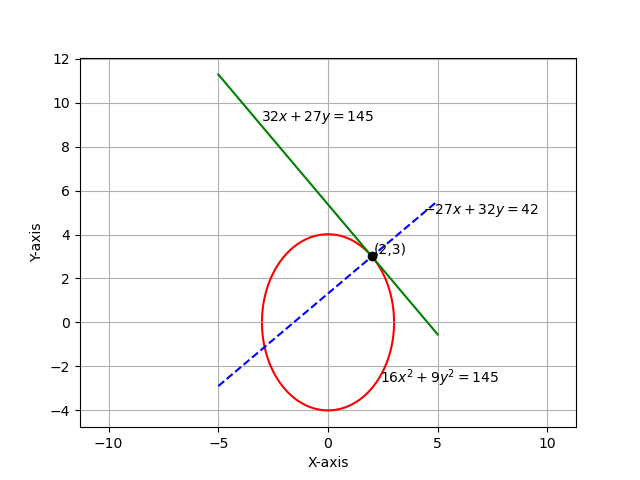
\includegraphics[width=0.7\linewidth]{figs/plot.png}
   \caption{Plot of the ellipse, tangent and normal}
   \label{}
\end{figure}

\end{document}
